\documentclass{article}
\usepackage[utf8]{inputenc} % un package
\usepackage[T1]{fontenc}      % un second package
\usepackage[francais]{babel}  % un troisième package
\usepackage{graphicx} %pour incorporer des figures

\title{Application de Test - Démonstration de fonctionnement de Rgtk}
\author{Alexandre Masson}
\date{16 Avril 2013}

\begin{document}

\maketitle
\newpage
\tableofcontents
\newpage

\section{Principe de l'application}
\subsection{Pourquoi faire cette application}
\paragraph{}
Ce projet de recherche devant se placer dans la continuité, nous allons réaliser une petite application pour pouvoir laisser à ceux qui nous succéderons, un voie à suivre pour implémenter Explorer3D avec RGtk, car nous l'avons déjà évoqué, RGtk semble être un package viable pour un portage sous R. 

\paragraph{} 
Nous allons donc réaliser une petite application Utilisant les principales fonctionnalités de RGtk. Cette application simple va pour le moment proposer une interface graphique pour pouvoir charger un fichier.\\
Dans ce contexte nous parlerons d'un moyen de pouvoir entrer le nom de fichier à charger, ainsi que des composants graphiques permettant de renseigner les différentes options de chargement disponibles sous R.

\paragraph{} 
Dans un second temps, il serait souhaitable de pouvoir visualiser les données que l'utilisateur souhaite charger.\\
Nous voudrions pouvoir afficher les données chargées dans la partie droite de l'écran, dans un "tableur", cela permettra à l'utilisateur de prévisualiser ses données. 

\paragraph{}
L'idéal serait dans un troisième temps de pouvoir lancer une fenêtre 3D avec les objets chargés, cela fera une connexion avec la partie visualisation 3D de ce TER.

\subsection{RGtk}
\paragraph{} 
Cette petite application ne fais pas partie des plus compliquées, toutefois elle demande la mise en place de plusieurs aspects de RGtk. On peux en effet noter que cette tache nous permet d'aborder les méthodes de placements des objets dans la fenêtre et donc de voir comment ce concept est géré sous RGtk.\\
Mais aussi comment mettre en place les différents composants graphiques tels que les boutons, les checkbox, et les champs texte.\\
De ces composants graphiques nait un besoin : gérer les événements. Nous allons donc au travers de cette application, explorer aussi ce coté de RGtk, et voir comment envoyer un signal quand un événement ce produit et comment appliquer des comportements à ces événements.\\

\newpage

\section{Comment fonctionne RGtk}
\subsection{Fenêtres et conteneurs}
\paragraph{} 
D'après ce que nous avons pu tester jusqu'à présent, RGtk se base sur des conteneur , qui sont soit verticaux( Vbox) soit horizontaux(Hbox ), et ces "cellules" s'imbriquent les unes dans les autres, elle même contenues dans une fenêtre (window) qui contient une frame, qui contient tout le contenu de la fenêtre (elle s’approcherait de l'"onglet" dans d'autres systèmes de création d'interfaces). C'est dans ces Box que nous pouvons ensuite ajouter des composants graphiques.\\

Dans la figure suivante, on peut voir la window et la frame (grâce au titre de la frame, RGtk affiche un cadre autour de la frame(l'onglet courant).\\

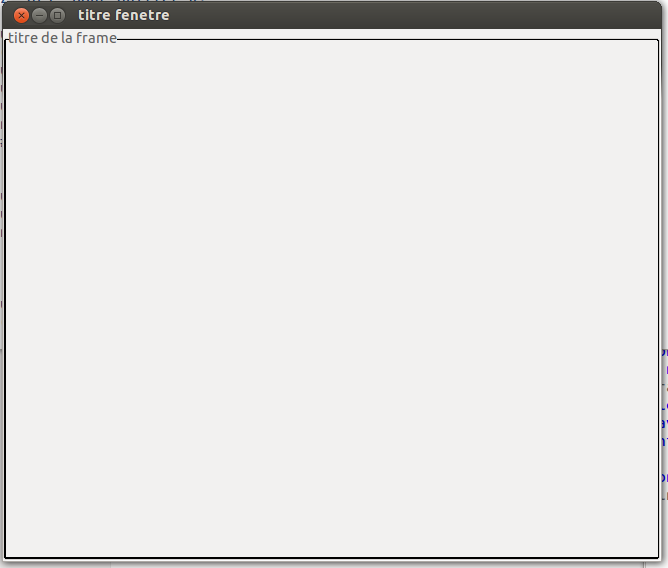
\includegraphics[scale=0.5]{fenetreVide.png}\\\\

\paragraph{} 
Pour obtenir la figure ci-dessus, il suffit du code suivant :\\

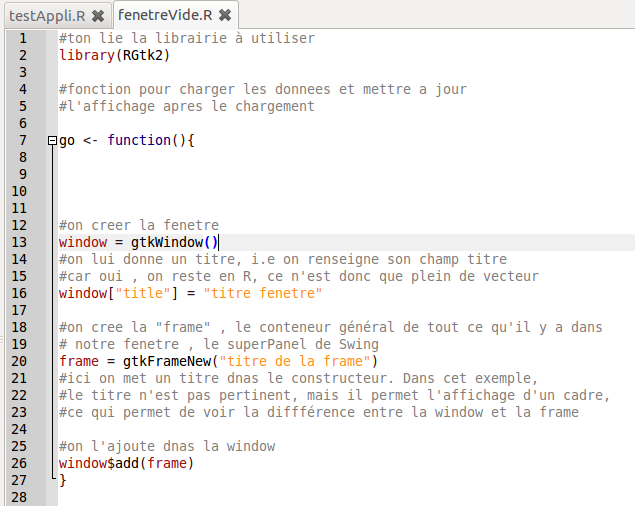
\includegraphics[scale=0.5]{exempleCode.png}

\subsection{Boutons, checkboxs, labels et Champs de texte}
\paragraph{} 
Nous allons maintenant présenter les boutons, checkboxs et autres gadgets pour interagir avec R depuis l'interface utilisateur. \\
Comme la plupart des systèmes de création d'interface graphique, RGtk propose un certain nombre de composant qu'il suffit de paramétrer, pour ensuite les ajouter dans une HBox ou VBox suivant l'alignement recherché.

\subsection{Événements }


\section{Utilité pour la suite}
\paragraph{}
Dans cette section, nous allons expliquer en quoi et pourquoi RGtk sera utile si l'on veux effectuer un portage d'Explorer3D. Nous essayerons de décrire quel composant répond à quel besoin, et surtout comment, en mettant en avant la manière d'arriver au résultats souhaité, une sorte de petit didacticiel pour permettre à ceux qui prendrons la suite de perdre le moins de temps possible à la découverte de cette technologie.
\end{document}